\section{SENSORES}
Los sensores son herramientas que detectan y responden a algún tipo de información del entorno físico. Existe una amplia gama de sensores utilizados en la vida diaria, que se clasifican según las cantidades y características que detectan.
\section{SENSORES INTERNOS}
\section{POSICION}
\section*{Encoder incremental}
Estos Pueden darnos información acerca de las revoluciones posición ángulo y posición. Este sensor envía un número de pulsos por revolución lo cual el encoder envía al controlador el cual contará el número de pulsos y calculará la posición actual a partir de estos impulsos. Estos son muy versátiles, pudiendo detectar la velocidad y sentido de giro de un motor, así como pueden ser montados directamente en un motor, eje u otro dispositivo giratorio.
	\section{Encoder Absoluto}
Estos detectan el movimiento rotativo a partir de incrementos angulares específicos. A diferencia de los encoders incrementales, en vez de enviar un impulso por cada ángulo de rotación, estos tienen un código específico por cada ángulo de giro por lo que el envío de un código es la referencia inequívoca de la posición. 
	\section{Potenciometro}
Un sensor del potenciómetro mide la distancia o el desplazamiento de un objeto en un movimiento lineal o rotatorio y lo convierte en una señal eléctrica. Estos funcionan\cite{TE_Potentiometer} a partir de una resistencia variable la cual a partir del movimiento mecánico del sensor cambia la resistividad del potenciómetro. Este cambio de resistividad puede ser después medido, y calcular el movimiento a partir de este. Existen tanto sensores de potenciómetro lineales como rotativos.\autoref{fig:potenciometro}.
	\begin{figure}[h]
		\centering
		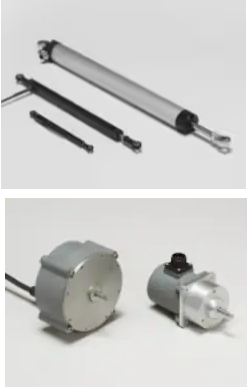
\includegraphics[width=0.3\linewidth]{img/potenciometro}
		\caption{imagen de sensor}
		\label{fig:potenciometro}
	\end{figure}
